\section{Introdução}

    \subsection{O que é a Internet?}

    Bilhões de dispositivos se conectam à Internet atualmente.

    \begin{itemize}[left=0.5cm, align=left, nosep]
        
        \item \textbf{Hosts (sistemas finais) :}  
        \begin{itemize}[left=0.5cm, nosep, label=$\hookrightarrow$]
            \item \underline{Exemplos:} smartphones, notebooks, máquinas servidoras, etc.
            \item Executam \textbf{aplicações de rede} e \textbf{interagem com o usuário}.
        \end{itemize}           
        
        \item \textbf{Packet switches (comutadores de pacotes) :}          
        \begin{itemize}[left=0.5cm, nosep, label=$\hookrightarrow$]
            \item Incluem \textbf{roteadores} e \textbf{switches}.
            \item Responsáveis por \underline{transportar pedaços de dados (pacotes)} de um ponto ao outro.
        \end{itemize}     
        
        \item \textbf{Communication links (enlaces de comunicação) :} 
        \begin{itemize}[left=0.5cm, nosep, label=$\hookrightarrow$]
            \item Recursos necessários para conectar dispositivos (finais, switches, roteadores, etc.).   
            \item Tipos : 
            \begin{itemize}[left=0.5cm, nosep, label=$-$]
                \item \textbf{Cabeados:} fibra óptica, cobre.  
                \item \textbf{Sem fio:} Wi-Fi, satélite.
            \end{itemize}
            \item \textbf{Taxa de transmissão:} também chamada de \underline{Banda}.
        \end{itemize}  
        
        \item \textbf{Redes :}   
        \begin{itemize}[left=0.5cm, nosep, label=$\hookrightarrow$]
            \item Coleção de dispositivos e roteadores sob uma \underline{gerência centralizada} por uma instituição.  
            \item \textbf{Tipos:}
            \begin{itemize}[left=0.5cm, nosep, label=$-$]
                \item \textbf{Públicas:} padrões abertos, como HTTP, Ethernet.  
                \item \textbf{Proprietárias:} mantidas por instituições privadas, como o Skype.
            \end{itemize}
        \end{itemize} 
        
        \item \textbf{IETF (Internet Engineering Task Force) :}
        \begin{itemize}[left=0.5cm, nosep, label=$\hookrightarrow$]
            \item Responsável por \underline{gerenciar e controlar os padrões da Internet}.  
            \item Cada padrão é lançado como um \textbf{RFC (Request for Comments)}. 
            \item Define e especifica as \textbf{características de um protocolo}. 
        \end{itemize}
        
        \item \textbf{Internet como infraestrutura de serviços :} 
        \begin{itemize}[left=0.5cm, nosep, label=$\hookrightarrow$]
            \item Provê serviços para \textbf{aplicações que executam em sistemas finais}.   
            \item \underline{Exemplos:} web, streaming de vídeo, e-mail, jogos, redes sociais, etc. 
        \end{itemize}
        
        \item \textbf{Interface de programação para aplicações distribuídas :} 
        \begin{itemize}[left=0.5cm, nosep, label=$\hookrightarrow$]
            \item Permite que uma aplicação \underline{envie mensagens pela Internet}. 
            \item Garante que o receptor consiga \underline{receber a mensagem de forma apropriada}.
        \end{itemize}
    \end{itemize}

    \subsection{O que é um Protocolo ?}
        $\bullet$ Um \textbf{protocolo} define o \underline{formato}, a \underline{ordem das mensagens} enviadas e recebidas entre entidades da rede, e as \textbf{ações a serem tomadas} ao receber ou transmitir uma mensagem.
    \subsection{Borda da Rede}

    \begin{itemize}[left=0.5cm, align=left, nosep]
        \item Composta pelos \textbf{sistemas finais} (\textbf{hosts}: clientes e servidores, geralmente em \textit{data centers}).
        \item A \textbf{conexão} desses dispositivos à rede é feita através das \textbf{redes de acesso} (\textit{sem fio ou cabeadas}).
        \item O restante da rede é chamado de \underline{núcleo da rede} — responsável pela interconexão de roteadores (a “rede de redes”).
    \end{itemize}

    \subsubsection*{Como conectar sistemas finais aos roteadores de borda ?}
    \begin{itemize}[left=0.5cm, align=left, nosep]
        \item \textbf{Redes de acesso residenciais}
        \item \textbf{Redes de acesso institucionais} (escolas, empresas)
        \item \textbf{Redes de acesso sem fio} (WiFi, 4G/5G)
    \end{itemize}

    \subsubsection*{Redes de Acesso}
    \begin{itemize}[left=0.5cm, align=left, nosep]
        \item \textbf{Taxa de transmissão} (\textbf{bits por segundo}) que o acesso permite — geralmente ligada à forma de compartilhamento do enlace e à capacidade de saída do roteador.
        \item O acesso é \textbf{dedicado} ou \textbf{compartilhado} entre os usuários ?
    \end{itemize}

    \subsubsection*{Exemplos de Redes de Acesso}

    \paragraph{TV a Cabo}
    \begin{itemize}[left=0.5cm, align=left, nosep]
        \item Utiliza o \textbf{divisor de frequência} ou \textbf{multiplexador FDM} (\textit{Frequency Division Multiplexing}) : \\ 
        \begin{itemize}[left=0.5cm, nosep, label=$\hookrightarrow$]
            \item Diferentes canais de transmissão em diferentes faixas de frequência.
        \end{itemize}    
    \end{itemize}

    \begin{figure}[H]
        \centering
        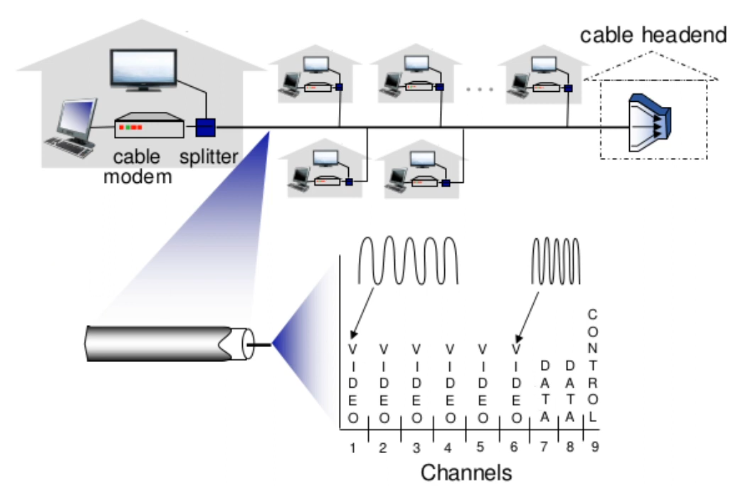
\includegraphics[width=0.6\textwidth]{img/cap-01/tv-a-cabo.png}
        \caption{Rede de acesso via TV a cabo (FDM).}
    \end{figure}

    \begin{figure}[H]
        \centering
        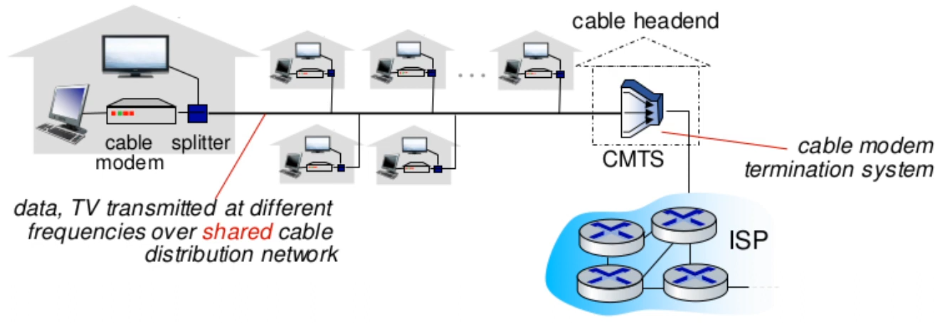
\includegraphics[width=0.6\textwidth]{img/cap-01/tv-a-cabo2.png}
        \caption{Arquitetura HFC híbrida coaxial-fibra.}
    \end{figure}
    
    \begin{itemize}[left=0.5cm, align=left, nosep]
        
        \item Utiliza-se \textbf{HFC (Hybrid Fiber Coaxial)}, uma solução híbrida : 
        \begin{itemize}[left=0.5cm, nosep, label=$\hookrightarrow$]
            \item O \textbf{cabo coaxial} vai até o usuário. 
            \item A \textbf{interconexão} da rede é feita usando \textbf{fibra óptica}. 
        \end{itemize} 
        
        \item \textbf{Assimétrica}: a capacidade de download e upload são diferentes.
        \item \textbf{Meio compartilhado}: o enlace é compartilhado entre vários usuários domésticos.
    \end{itemize}

    \paragraph{Rede baseada em DSL (\textit{Digital Subscriber Line})}
    \begin{itemize}[left=0.5cm, align=left, nosep]
        \item Utiliza os \textbf{cabos telefônicos} como infraestrutura de enlace.
        \item A conexão \underline{não é compartilhada}.
        \item \textbf{Assimétrica} — download e upload possuem taxas diferentes.
    \end{itemize}

    \begin{figure}[H]
        \centering
        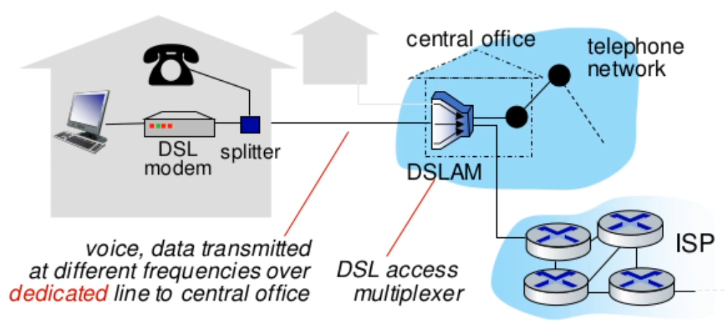
\includegraphics[width=0.6\textwidth]{img/cap-01/dsl.png}
        \caption{Rede DSL utilizando a infraestrutura telefônica.}
    \end{figure}

    {\textbf{Rede Doméstica}}

    \begin{figure}[H]
        \centering
        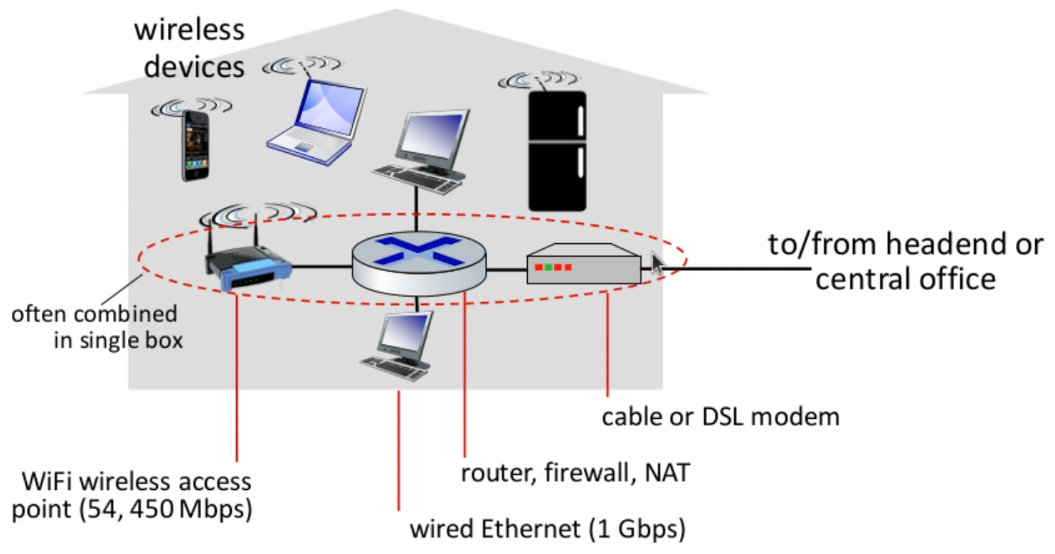
\includegraphics[width=0.4\textwidth]{img/cap-01/rede-domestica.png}
        \caption{Exemplo de rede doméstica.}
    \end{figure}

    \paragraph{Redes de Acesso Sem Fio (Wireless)}
    \begin{itemize}[left=0.5cm, align=left, nosep]
        \item O \textbf{roteador de borda} é conectado a um \textbf{ponto de acesso}.
        \item \textbf{Locais}: alcance reduzido (domésticas, empresas) — \textbf{WiFi}.
        \item \textbf{Longas distâncias}: móveis (4G/5G), com pontos de acesso em \textbf{torres}, menor capacidade de transmissão.
    \end{itemize}

    \paragraph{Redes de Acesso Institucionais}
    \begin{itemize}[left=0.5cm, align=left, nosep]
        \item Utilizadas em \textbf{universidades}, \textbf{empresas}, etc.
        \item Maior complexidade de interconexão — acesso sem fio conectado a switches e roteadores.
        
        \item Tecnologias utilizadas :
        \begin{itemize}[left=0.5cm, nosep, label=$\hookrightarrow$]
            \item \textbf{Ethernet} 
            \item \textbf{WiFi}
        \end{itemize} 
    
    \end{itemize}

    \begin{figure}[H]
        \centering
        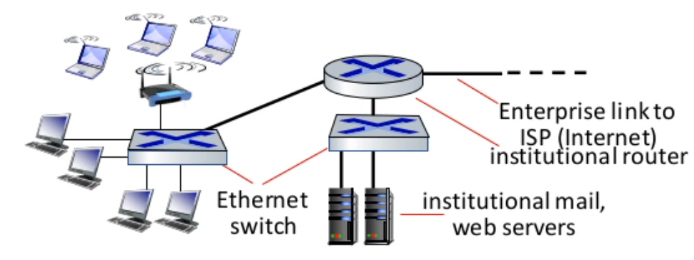
\includegraphics[width=0.5\textwidth]{img/cap-01/rede-institucional.png}
        \caption{Rede de acesso institucional.}
    \end{figure}

    \subsubsection*{Hosts (Sistemas Finais)}
    \begin{itemize}[left=0.5cm, align=left, nosep]
        \item Quando o \textbf{host} tem conectividade, é possível enviar \textbf{pacotes de dados} até o destinatário.
        
        \item \textbf{Função de envio :} 
        \begin{itemize}[left=0.5cm, nosep, label=$\hookrightarrow$]
            \item Pega uma \textbf{mensagem} de uma aplicação.
            \item Quebra essa mensagem em \textbf{pacotes menores} de tamanho $L$ bits.
            \item Esses pacotes são transmitidos a uma taxa de transmissão $R$ (\textbf{bits/s}), correspondente à capacidade do enlace.
        \end{itemize}      
        
        \item \underline{Tempo de retardo (delay)} = tempo necessário para transmitir um pacote:  
        \[
        \text{delay} = \frac{L (\text{bits})}{R (\text{bits/s})}
        \]
    \end{itemize}

    \subsubsection*{Links (Enlaces)}
    \begin{itemize}[left=0.5cm, align=left, nosep]
        \item Utilizados para a \textbf{interconexão de dispositivos}.
        \item Caracterizados por propriedades físicas.
        \item O \textbf{bit} é propagado entre transmissor e receptor.
        
        \item \textbf{Tipos de enlaces :}
        \begin{itemize}[left=0.5cm, nosep, label=$\hookrightarrow$]
            \item \textbf{Guiados}: sinal se propaga em meio sólido (fibra óptica, cabos coaxiais, par trançado).
            \item \textbf{Não guiados}: sinal se propaga de forma livre (ondas eletromagnéticas). 
        \end{itemize}     
    \end{itemize}

    \paragraph{Cabos Par Trançado (Twisted Pair - TP)} 
    \begin{itemize}[left=0.5cm, align=left, nosep]    
        \item Categorias mais comuns: \textbf{Cat 5}, \textbf{Cat 6}.
    \end{itemize}

    \begin{figure}[H]
        \centering
        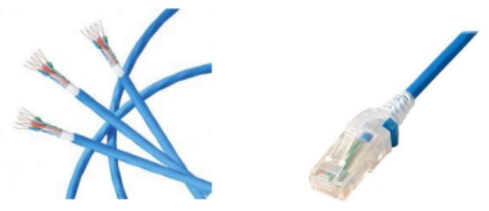
\includegraphics[width=0.35\textwidth]{img/cap-01/cabos-tp.png}
        \caption{Cabos Par Trançado (Twisted Pair).}
    \end{figure}

    \paragraph{Cabos Coaxiais}
    \begin{itemize}[left=0.5cm, align=left, nosep]
        \item Dois condutores de cobre concêntricos.
        \item \textbf{Bidirecional}: transmite e recebe dados simultaneamente.
        \item Suporta \textbf{conexão de banda larga} — coexistência de múltiplas frequências no mesmo cabo.
    \end{itemize}

    \begin{figure}[H]
        \centering
        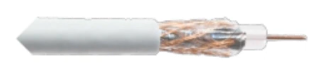
\includegraphics[width=0.35\textwidth]{img/cap-01/cabo-coaxial.png}
        \caption{Estrutura de um cabo coaxial.}
    \end{figure}

    \paragraph{Cabos de Fibra Óptica}
    \begin{itemize}[left=0.5cm, align=left, nosep]
        \item Feitos de \textbf{vidro}.
        \item Transmissão em \textbf{alta velocidade} e \textbf{longa distância}.
        \item \textbf{Taxa de erro muito baixa}, dispensando regeneração do sinal.
        \item Imunes a \textbf{ruídos eletromagnéticos}.
    \end{itemize}

    \begin{figure}[H]
        \centering
        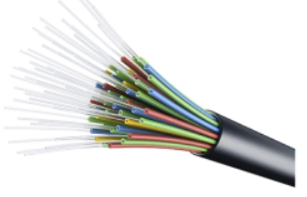
\includegraphics[width=0.35\textwidth]{img/cap-01/fibra-optica.png}
        \caption{Cabo de fibra óptica.}
    \end{figure}

    \paragraph{Transmissão via Rádio}
    \begin{itemize}[left=0.5cm, align=left, nosep]
        \item Sinal transmitido no \textbf{espectro eletromagnético}.
        \item Comunicação \textbf{sem fio} e geralmente em modo \textbf{broadcast} (difusão).
        \item Operação \textbf{half-duplex}: alterna entre receber e enviar informações.
        \item \textbf{Problemas comuns de transmissão :}
        \begin{itemize}[left=0.5cm, nosep, label=$\hookrightarrow$]
            \item Reflexão 
            \item Obstrução por objetos 
            \item Interferência 
        \end{itemize} 
        
        \item \textbf{Tipos de transmissão via rádio :} 
        \begin{itemize}[left=0.5cm, nosep, label=$\hookrightarrow$]
            \item Micro-ondas terrestres 
            \item \textbf{Wireless LAN} (WiFi) 
            \item \textbf{Sem fio de longo alcance} (4G/5G) 
            \item \textbf{Satélite} — possui \underline{retardo de transmissão elevado}.
        \end{itemize} 
    \end{itemize}

    \subsection{Núcleo da Rede}

    \begin{itemize}[left=0.5cm, align=left, nosep]
        \item Parte \textbf{central da rede}, responsável por interconectar as redes de acesso.
        \item É composta por uma \textbf{malha de roteadores interconectados} que realizam o \textbf{encaminhamento de pacotes de dados} gerados pelos sistemas finais.
    \end{itemize}

    \subsubsection*{Comutação de Pacotes (\textit{Packet Switching})}
    \begin{itemize}[left=0.5cm, align=left, nosep]
        \item O \textbf{sistema final} divide a \textbf{mensagem da aplicação} em \textbf{pacotes}.
        \item Esses pacotes são encaminhados \underline{roteador a roteador}, seguindo um caminho até o destino.
        \item Cada pacote é transmitido utilizando \textbf{toda a capacidade do enlace} entre os roteadores.
    \end{itemize}

    \begin{figure}[H]
        \centering
        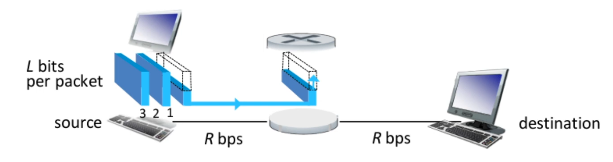
\includegraphics[width=0.55\textwidth]{img/cap-01/retardo.png}
        \caption{Encaminhamento de pacotes e retardo na transmissão.}
    \end{figure}

    \begin{itemize}[left=0.5cm, align=left, nosep]
        \item Cada pacote passa por uma série de roteadores desde a origem até o destino.
        \item Em cada roteador é necessário que o pacote seja \textbf{recebido completamente} antes de ser retransmitido.
        \item \underline{Delay fim-a-fim}: $2L/R$ (assumindo delay de propagação nulo).
        \item \textbf{Exemplo:} $L = 10$ Kbits, $R = 100$ Mbps $\Rightarrow$ cada salto de transmissão leva $0.1$ ms.
    \end{itemize}

    \paragraph{Atrasos e Perdas (\textit{Queueing Delay, Loss})}
    \begin{itemize}[left=0.5cm, align=left, nosep]
        \item Quando a \textbf{taxa de chegada} de pacotes em um roteador excede a \textbf{taxa de saída}, ocorre o \underline{enfileiramento}.
        \item Pacotes são \textbf{enfileirados} aguardando o enlace ficar livre — adicionando retardo ao processo de transmissão fim a fim.
        \item Caso a fila de saída esteja cheia, os pacotes são \textbf{descartados (perdidos)}.
    \end{itemize}

    \begin{figure}[H]
        \centering
        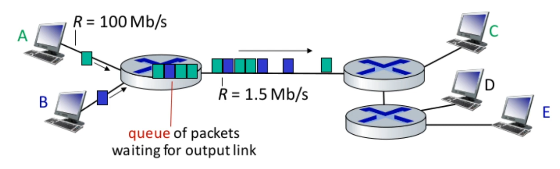
\includegraphics[width=0.45\textwidth]{img/cap-01/fila-e-perda.png}
        \caption{Fila de pacotes e perdas em roteadores.}
    \end{figure}

    \subsubsection*{Funções Principais do Núcleo da Rede}
    \begin{itemize}[left=0.5cm, align=left, nosep]
        \item \textbf{Encaminhamento (Forwarding):} ação \underline{local} — move pacotes do enlace de entrada para o enlace de saída apropriado.
        \item \textbf{Roteamento (Routing):} ação \underline{global} — define os caminhos de origem a destino dentro da rede, utilizando \textbf{algoritmos de roteamento}.
    \end{itemize}

    \begin{figure}[H]
        \centering
        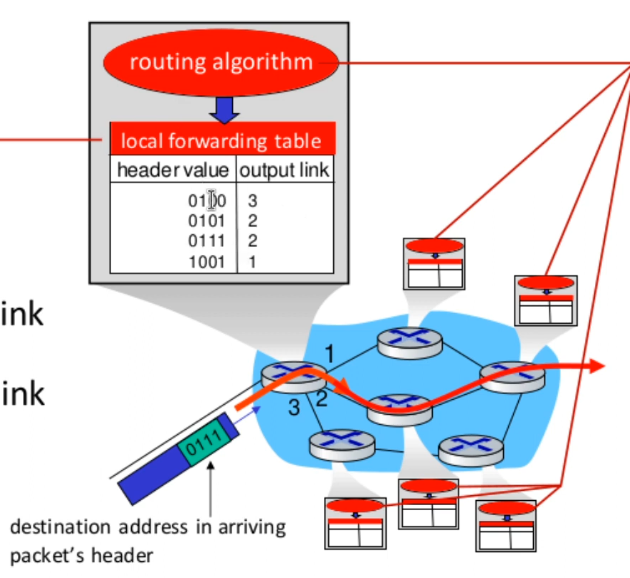
\includegraphics[width=0.35\textwidth]{img/cap-01/encaminhamento-roteamento.png}
        \caption{Diferença entre encaminhamento e roteamento.}
    \end{figure}

    \subsubsection*{Alternativa: Comutação por Circuito}
    \begin{itemize}[left=0.5cm, align=left, nosep]
        \item Na comutação por circuito, existe uma \textbf{etapa inicial de conexão} onde :        
        \begin{itemize}[left=0.5cm, nosep, label=$\hookrightarrow$]
            \item É definida a rota completa do início ao fim. 
            \item São \textbf{alocados recursos} nos roteadores ao longo do caminho. 
            \item Cada roteador envolvido armazena informação sobre essa rota. 
        \end{itemize} 
        \item Os pacotes transportam a informação sobre o \textbf{circuito virtual} ao qual pertencem.
    \end{itemize}

    \begin{figure}[H]
        \centering
        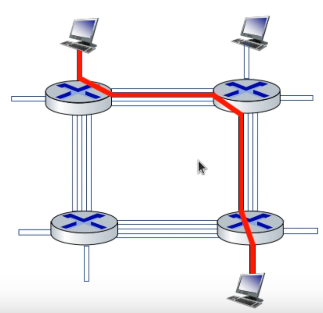
\includegraphics[width=0.25\textwidth]{img/cap-01/comutacao-circuitos.png}
        \caption{Comutação por circuito.}
    \end{figure}

    \paragraph{Técnicas de Multiplexação}
    \begin{itemize}[left=0.5cm, align=left, nosep]
        \item \textbf{Frequency Division Multiplexing (FDM) :} 
        \begin{itemize}[left=0.5cm, nosep, label=$\hookrightarrow$]
            \item Divide a capacidade do enlace em \textbf{faixas de frequência}. 
            \item Cada faixa é dedicada a um usuário, transmitindo até a taxa máxima da sua banda. 
        \end{itemize} 
        
        \begin{figure}[H]
            \centering
            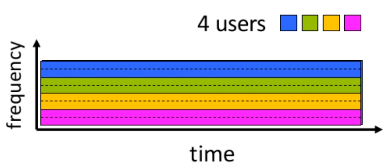
\includegraphics[width=0.35\textwidth]{img/cap-01/multiplexicacao-por-frequencia.png}
            \caption{Multiplexação por frequência (FDM).}
        \end{figure}

        \item \textbf{Time Division Multiplexing (TDM) :} 
        \begin{itemize}[left=0.5cm, nosep, label=$\hookrightarrow$]
            \item Divide o tempo de transmissão em \textbf{intervalos (slots)}. 
            \item Cada usuário transmite à taxa total do enlace durante o seu slot de tempo.
        \end{itemize}     
        
        \begin{figure}[H]
            \centering
            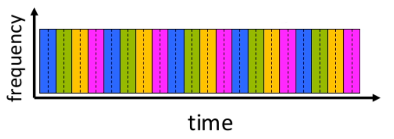
\includegraphics[width=0.35\textwidth]{img/cap-01/multiplexicacao-por-tempo.png}
            \caption{Multiplexação por tempo (TDM).}
        \end{figure}
    \end{itemize}

    \paragraph{Comparação: Comutação de Pacotes vs. Comutação de Circuitos}
    \begin{itemize}[left=0.5cm, align=left, nosep]
        \item Ambas possuem a mesma \textbf{taxa de transmissão nominal}.
        \item A \textbf{comutação de pacotes} permite que mais usuários utilizem a rede simultaneamente.
        \item É mais eficiente para \textbf{“bursty data”} (rajadas de dados) :     
        \begin{itemize}[left=0.5cm, nosep, label=$\hookrightarrow$]
            \item Melhor \textbf{compartilhamento de recursos}.
            \item Operação mais \textbf{simples}, sem necessidade de estabelecimento de chamada. 
        \end{itemize} 
        \item \textbf{Problema :} Ausência de controle de congestionamento. 
        \begin{itemize}[left=0.5cm, nosep, label=$\hookrightarrow$]
            \item Pode causar aumento de retardo e perda de pacotes devido ao transbordo das filas. 
            \item Protocolos específicos são utilizados para controle de congestionamento. 
        \end{itemize} 
        \item Aplicações como \textbf{vídeo/áudio streaming} ainda utilizam comutação de circuitos.
    \end{itemize}

    \subsubsection*{Estrutura da Internet}
    
    \begin{itemize}[left=0.5cm, align=left, nosep]
        \item Os \textbf{hosts} se conectam à Internet por meio de \textbf{provedores de acesso (ISPs)} :
        \begin{itemize}[left=0.5cm, nosep, label=$\hookrightarrow$]
            \item Domésticos, empresariais ou institucionais.
        \end{itemize} 

        \item Esses provedores precisam se \textbf{interconectar} para permitir comunicação entre seus clientes.
        \item Isso resultou em uma rede de \textbf{alta complexidade}, moldada por \textbf{decisões econômicas e políticas}.
    \end{itemize}

    \begin{figure}[H]
        \centering
        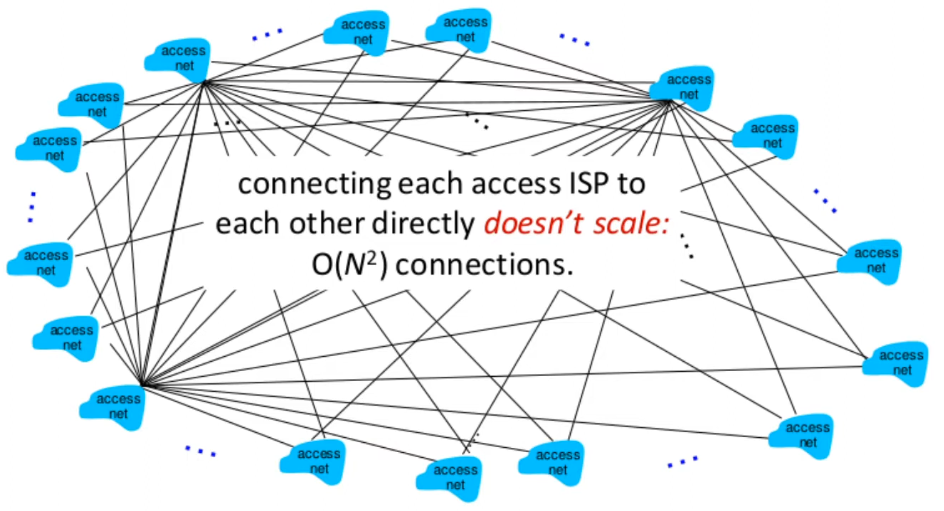
\includegraphics[width=0.4\textwidth]{img/cap-01/infraestrutura1.png}
        \caption{Evolução da infraestrutura da Internet.}
    \end{figure}

    \paragraph{Hierarquização da Conexão}
    \begin{itemize}[left=0.5cm, align=left, nosep]
        \item Solução: criar um \textbf{provedor de acesso global}.
        \item Provedores locais se conectam a ele, estabelecendo uma relação \textbf{econômica} (pagamento pelo uso do serviço de trânsito).
    \end{itemize}

    \begin{figure}[H]
        \centering
        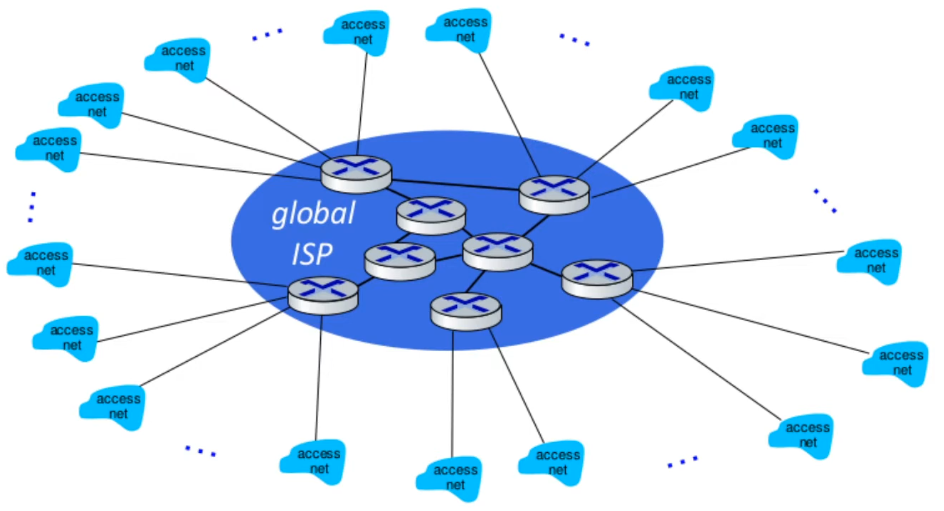
\includegraphics[width=0.4\textwidth]{img/cap-01/infraestrutura2.png}
        \caption{Conexão hierárquica entre provedores locais e globais.}
    \end{figure}

    \begin{itemize}[left=0.5cm, align=left, nosep]
        \item Com o tempo, surgiu \textbf{concorrência} tanto por questões econômicas quanto geográficas.
    \end{itemize}

    \begin{figure}[H]
        \centering
        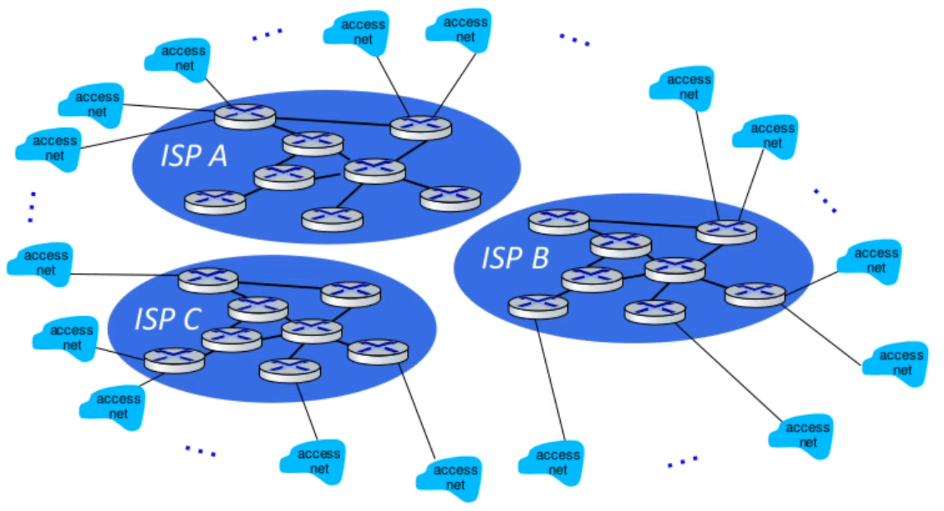
\includegraphics[width=0.4\textwidth]{img/cap-01/infraestrutura3.png}
        \caption{Concorrência e distribuição geográfica de provedores.}
    \end{figure}

    \paragraph{Peering e Pontos de Troca de Tráfego}
    \begin{itemize}[left=0.5cm, align=left, nosep]
        \item A conexão entre provedores locais ocorre por meio de : 
        \begin{itemize}[left=0.5cm, nosep, label=$\hookrightarrow$]
            \item \textbf{Peering físico (peering link)} 
            \item \textbf{Pontos de Troca de Tráfego (IXP)}
        \end{itemize}     
    \end{itemize}

    \begin{figure}[H]
        \centering
        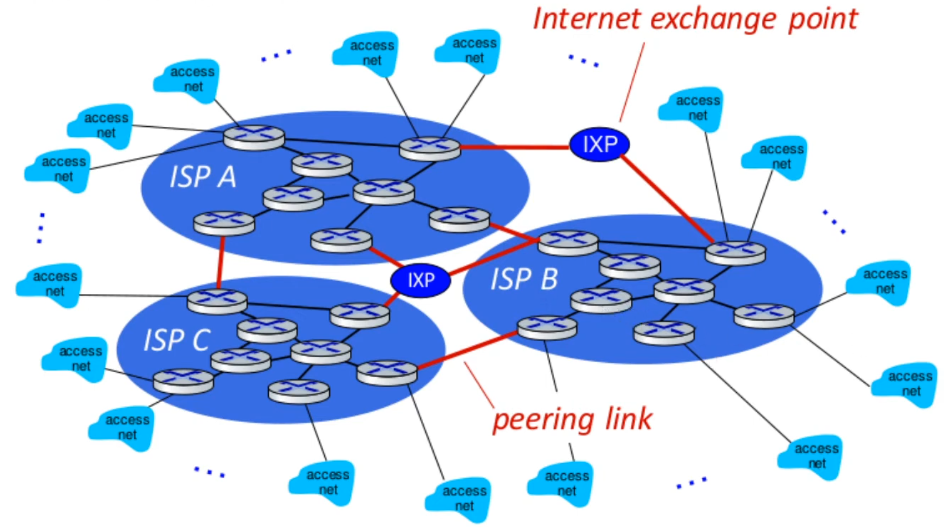
\includegraphics[width=0.4\textwidth]{img/cap-01/infraestrutura4.png}
        \caption{Conexão entre provedores locais e IXP.}
    \end{figure}

    \paragraph{Provedores Regionais e Globais}
    \begin{itemize}[left=0.5cm, align=left, nosep]
        \item Devido à distância geográfica entre provedores globais e locais, surgiram \textbf{provedores regionais}.
        \item Grandes provedores de conteúdo (\textbf{Google, Microsoft, etc.}) se conectam diretamente aos provedores globais.
    \end{itemize}

    \begin{figure}[H]
        \centering
        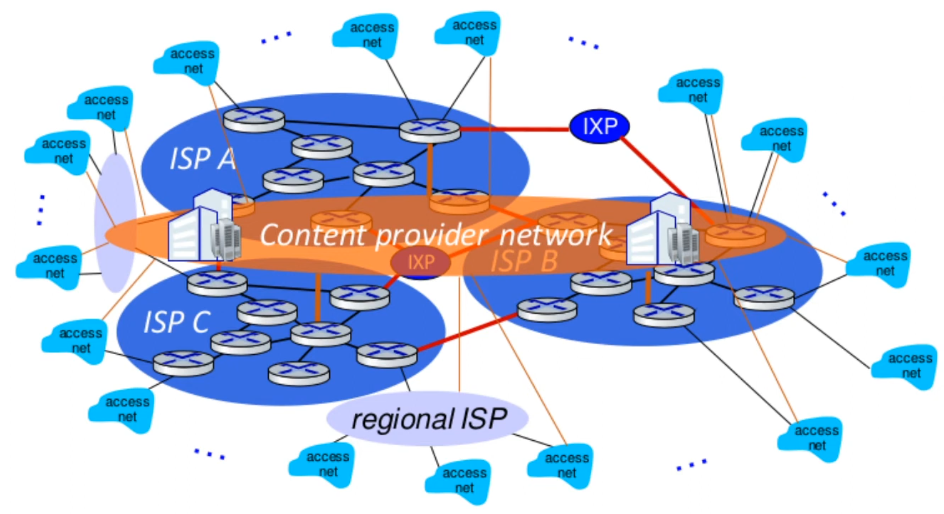
\includegraphics[width=0.4\textwidth]{img/cap-01/infraestrutura5.png}
        \caption{Conexão de provedores de conteúdo com provedores globais.}
    \end{figure}

    \vspace{1cm}
    \textbf{Hierarquia da Internet}

    \begin{figure}[H]
        \centering
        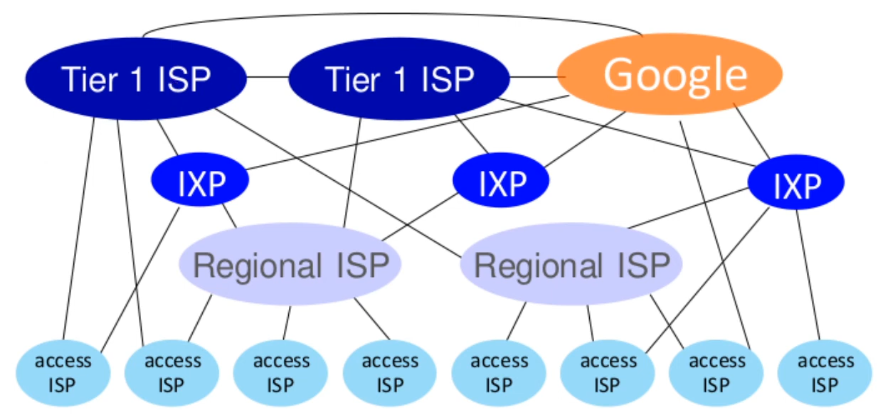
\includegraphics[width=0.4\textwidth]{img/cap-01/hierarquia.png}
        \caption{Hierarquia dos provedores de acesso à Internet.}
    \end{figure}

   \subsection{Performance}

    \begin{itemize}[left=0.5cm, align=left, nosep]
        
        \item \textbf{Como ocorre a perda e o retardo de pacotes ?} 
        \begin{itemize}[left=0.5cm, nosep, label=$\hookrightarrow$]
            \item Pacotes enfileirados esperam a sua vez de serem transmitidos. 
            \item \textbf{Retardo de enfileiramento}: \underline{tempo que um pacote aguarda na fila} para ser transmitido. 
            \item \textbf{Retardo de transmissão}: \underline{tempo que leva para transmitir os bits} no enlace. 
            \item Se a \textbf{taxa de chegada} no enlace (temporariamente) excede a capacidade de saída, ocorre a \textbf{perda de pacotes}. 
        \end{itemize} 
        
        \begin{center}
            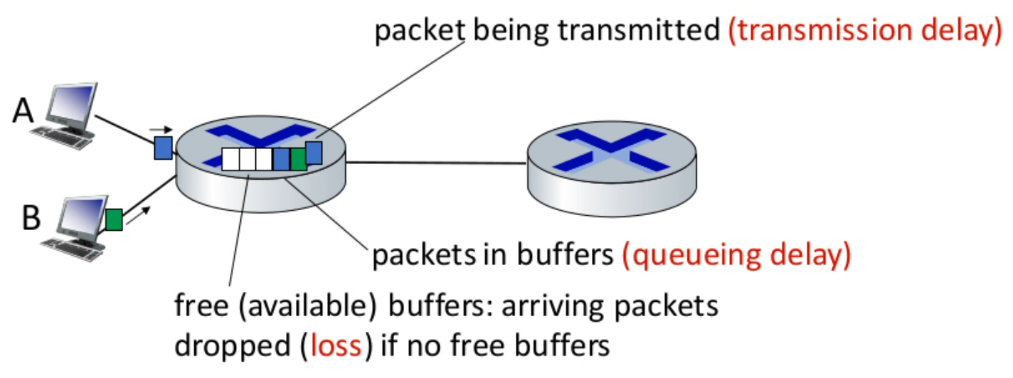
\includegraphics[width=0.5\textwidth]{img/cap-01/delay1.png}
        \end{center}

        \item \textbf{Retardo do Pacote: 4 Causas}
        \begin{itemize}[left=0.5cm, nosep, label=$\hookrightarrow$]
            \item O retardo ocorre a cada nó (ou salto) na rede : 
        \end{itemize} 
        
        \begin{center}
            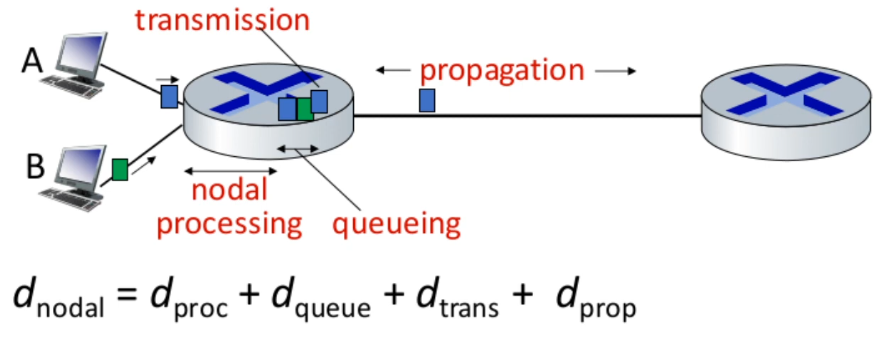
\includegraphics[width=0.45\textwidth]{img/cap-01/delay2.png}
        \end{center}

        \item \textbf{Componentes do Retardo :}
            
            \begin{itemize}[left=0.5cm, nosep, label=$\hookrightarrow$]
                \item \textbf{$d_{proc}$ : Retardo de Processamento do Nó}
                \begin{itemize}[left=0.5cm, nosep, label=$-$]
                    \item Tempo gasto pelo roteador para processar o pacote que acabou de chegar.
                    \item Envolve tarefas como:
                    \begin{itemize}[left=0.5cm, nosep, label=$\blacktriangleright$]
                        \item Conferir a integridade do pacote.
                        \item Verificar o endereço de saída do pacote.
                    \end{itemize}
                    \item Geralmente menor que 1 ms.
                \end{itemize}
            
                \item \textbf{$d_{queue}$ : Retardo de Enfileiramento} 
                \begin{itemize}[left=0.5cm, nosep, label=$-$]
                    \item Tempo que o pacote aguarda na fila antes da transmissão.
                    \item Depende do \textbf{nível de congestionamento} no roteador.
                \end{itemize}
                
                \item \textbf{$d_{trans}$ : Retardo de Transmissão}
                \begin{itemize}[left=0.5cm, nosep, label=$-$]
                    \item Tempo necessário para transmitir um pacote no enlace.
                    \item Dados : $L = \text{tamanho do pacote (bits)}$, $R = \text{taxa de transmissão (bps)}$
                    \item Fórmula : $\boxed{d_{trans} = \frac{L}{R}}$
                \end{itemize}

                \item \textbf{$d_{prop}$ : Retardo de Propagação}
                \begin{itemize}[left=0.5cm, nosep, label=$-$]
                    \item Tempo necessário para que os bits do pacote \underline{propaguem até o destino}.
                    \item $d = \text{comprimento do enlace}$, $s = \text{velocidade de propagação} \approx 2 \times 10^8 \text{ m/s}$
                    \item Fórmula : $\boxed{d_{prop} = \frac{d}{s}}$
                \end{itemize}
            
            \end{itemize} 
                        
        \item \textbf{Exemplo: Caravanas de Carros}
            
            \begin{itemize}[left=0.5cm, nosep, label=$\hookrightarrow$]
                \item Analogia :
                \begin{itemize}[left=0.5cm, nosep, label=$-$]
                    \item \textbf{1 Carro} $\rightarrow$ 1 \textbf{bit}.
                    \item \textbf{Caravana} $\rightarrow$ \textbf{pacote}.
                    \item \textbf{Pedágio} $\rightarrow$ \textbf{roteador}.
                    \item \textbf{Estrada} $\rightarrow$ \textbf{enlace}.
                \end{itemize}

                \item O pedágio leva 12 s para atender cada carro (tempo de transmissão). 
                \item A estrada tem pedágios a cada 100 km. 
                \item Um carro se propaga a 100 km/h. 
                \item \textbf{Pergunta 1:} Quanto tempo levaria para a caravana de 10 carros chegar ao 2º pedágio ? 
                \begin{itemize}[left=0.5cm, nosep, label=$-$]
                    \item Tempo de transmissão: $12 \times 10 = 120$ s.
                    \item Tempo de propagação: $100$ km / $100$ km/h = 1 h.
                    \item Tempo total: \textbf{62 minutos}.
                \end{itemize}

                \item \textbf{Pergunta 2:} Se os carros se propagam a 1000 km/h e o pedágio leva 1 min por carro? 
                \begin{itemize}[left=0.5cm, nosep, label=$-$]
                    \item Tempo de propagação: 6 min.
                    \item O primeiro carro chega ao segundo pedágio após 7 min, antes de todos terminarem no primeiro pedágio.
                \end{itemize}
            \end{itemize} 
                        
            \begin{center}
                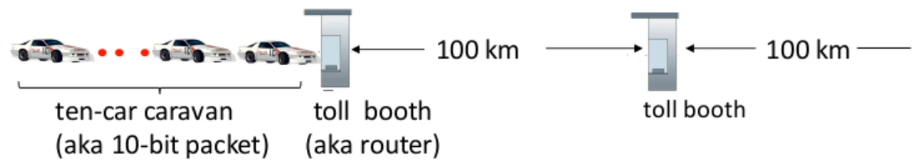
\includegraphics[width=0.7\textwidth]{img/cap-01/carro-pedagio.png}
            \end{center}

        \end{itemize}

    \subsubsection*{Revisão: Retardo de Enfileiramento}
        \begin{itemize}[left=0.5cm, align=left, nosep]
            \item $R = \text{Capacidade de transmissão (bps)}$ 
            \item $L = \text{Tamanho do pacote (bits)}$ 
            \item $a = \text{Taxa de chegada (pacotes/s)}$
            \begin{itemize}[left=0.5cm, nosep, label=$\hookrightarrow$]
                \item $\frac{La}{R} \approx 0$: Retardo pequeno.
                \item $\frac{La}{R} \rightarrow 1$: Retardo grande.
                \item $\frac{La}{R} > 1$: \underline{taxa de chegada maior que a capacidade de transmissão}, retardo tende ao infinito.
            \end{itemize}
        \end{itemize}
        
        \begin{center}
            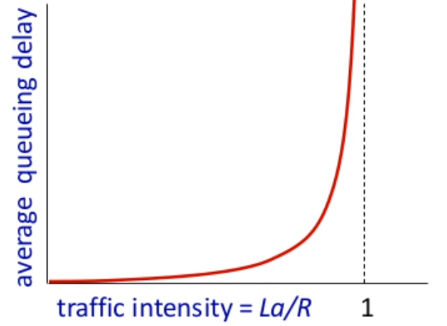
\includegraphics[width=0.4\textwidth]{img/cap-01/retardo-de-enfileiramento.png}
        \end{center}

        \begin{itemize}[left=0.5cm, align=left, nosep]
            
            \item \textbf{Exemplo Real : \texttt{traceroute}}
            \begin{itemize}[left=0.5cm, nosep, label=$\hookrightarrow$]
                \item Programa que permite \underline{avaliar cada roteador} ao longo da rota seguida pelos pacotes.
                \item Mostra o \textbf{tempo de ida e volta (RTT)} de cada salto.  
            \end{itemize}
        
            \begin{center}
                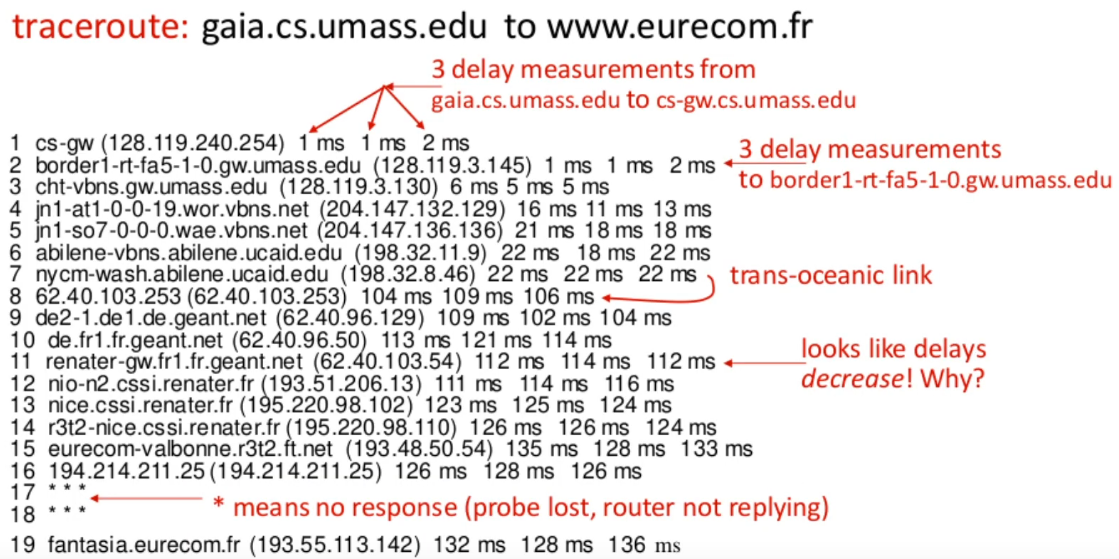
\includegraphics[width=0.55\textwidth]{img/cap-01/traceroute-exemplo.png}
            \end{center}
        
            \item \textbf{Perda de Pacotes}
            \begin{itemize}[left=0.5cm, nosep, label=$\hookrightarrow$]
                \item A fila (\textbf{buffer}) precede um enlace de saída.
                \item Quando a fila está cheia, o pacote é \underline{descartado}.
                \item Pacotes perdidos precisam ser \textbf{retransmitidos}.
            \end{itemize}

            \begin{center}
                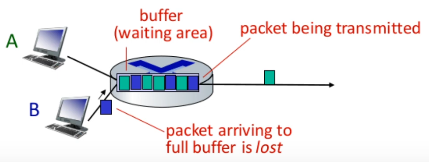
\includegraphics[width=0.3\textwidth]{img/cap-01/perda-de-pacotes.png}
            \end{center}
            
            \item \textbf{Vazão (Throughput)}
            \begin{itemize}[left=0.5cm, nosep, label=$\hookrightarrow$]
                \item \textbf{Throughput}: \underline{taxa de transmissão efetiva} percebida por uma conexão.
                \item Tipos:
                \begin{itemize}[left=0.5cm, nosep, label=$-$]
                    \item \textbf{Instantânea}: medida em um determinado instante.
                    \item \textbf{Média}: média ao longo de um período.
                \end{itemize}
                \item A vazão é sempre limitada pelo \textbf{link gargalo}.
            \end{itemize}
        
            \begin{center}
                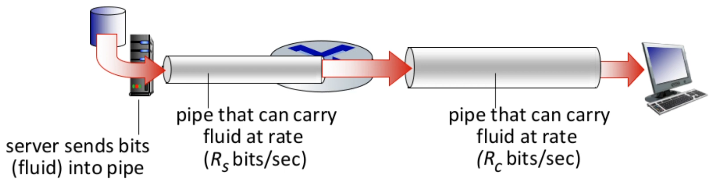
\includegraphics[width=0.4\textwidth]{img/cap-01/vazao.png}
            \end{center}

            \begin{center}
                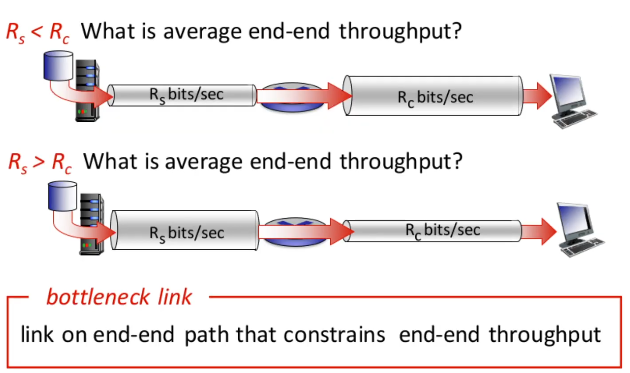
\includegraphics[width=0.4\textwidth]{img/cap-01/exemplo-vazao.png}
            \end{center}

            \begin{center}
                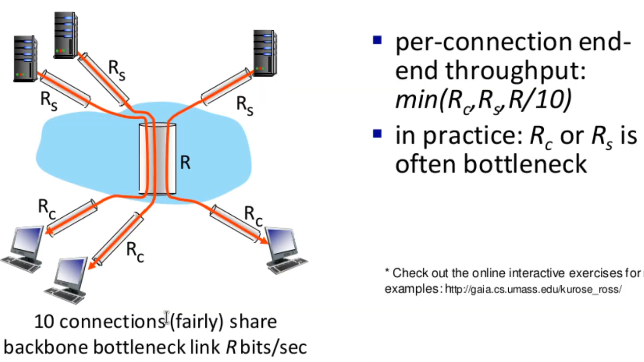
\includegraphics[width=0.4\textwidth]{img/cap-01/exemplo-vazao2.png}
            \end{center}
        
        \end{itemize} 
        
    \subsection{Camadas de Protocolos e Modelos de Serviços}

    \begin{itemize}[left=0.5cm, align=left, nosep]
        \item \textbf{Questão inicial:} Existia alguma maneira de organizar a estrutura da Internet?
        \item \textbf{Exemplo: Organização para Viajar de Avião} 
            \begin{itemize}[left=0.5cm, nosep, label=$\hookrightarrow$]
                \item Uma viagem de avião envolve uma série de etapas e serviços distintos.
                \item Cada etapa pode ser vista como uma \textbf{camada}, responsável por uma parte específica do processo.
            \end{itemize} 
        
        \begin{figure}[H]
            \centering
            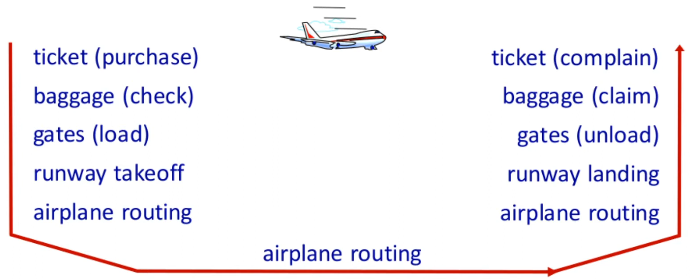
\includegraphics[width=0.4\textwidth]{img/cap-01/exemplo-aviao.png}
            \caption{Organização em etapas de uma viagem de avião.}
        \end{figure}

        \item \textbf{Camadas :}
            \begin{itemize}[left=0.5cm, nosep, label=$\hookrightarrow$]
                \item Cada camada implementa um \textbf{serviço} específico.
                \item Cada camada tem uma \textbf{contrapartida} tanto na origem quanto no destino.
            \end{itemize} 
    
        \begin{figure}[H]
            \centering
            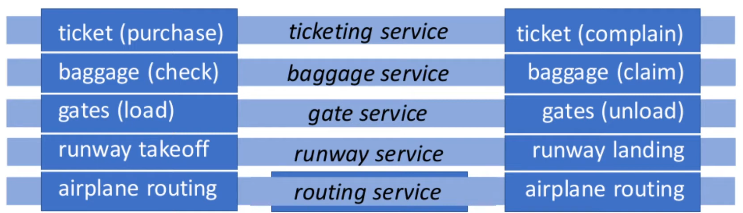
\includegraphics[width=0.4\textwidth]{img/cap-01/exemplo-aviao2.png}
            \caption{Camadas de serviço e suas contrapartidas.}
        \end{figure}

        \item \textbf{Por que usar camadas ?} 
            \begin{itemize}[left=0.5cm, nosep, label=$\hookrightarrow$]
                \item A ideia surge naturalmente em sistemas complexos. 
                \item \textbf{Abstrai} partes do sistema em diferentes camadas. 
                \item Cada camada deve ser \textbf{bem definida} e possuir uma \textbf{interface clara}. 
                \item Facilita a \textbf{modularização}, \textbf{manutenção} e \textbf{atualização} do sistema. 
                \item \underline{Problema:} pode haver \textbf{redundância de ações} entre camadas. 
            \end{itemize} 
        
        \item \textbf{Pilha de Protocolos da Internet (TCP/IP)}
            \begin{itemize}[left=0.5cm, nosep, label=$\hookrightarrow$]    
                
                \item \textbf{Aplicação :} Suporta as aplicações que estão executando nos sistemas finais.
                \begin{itemize}[left=0.5cm, nosep, label=$-$]
                    \item Exemplos: \texttt{HTTP}, \texttt{SMTP}, \texttt{IMAP}.
                \end{itemize}
                
                \item \textbf{Transporte :} Responsável pela \textbf{transferência de pacotes entre processos} que estão executando nos sistemas finais.
                \begin{itemize}[left=0.5cm, nosep, label=$-$]
                    \item Exemplos: \texttt{UDP}, \texttt{TCP}.
                \end{itemize}
                
                \item \textbf{Rede :} Faz o \textbf{roteamento dos pacotes} da origem até o destino.
                \begin{itemize}[left=0.5cm, nosep, label=$-$]
                    \item Exemplos: \texttt{IP}, \texttt{Protocolos de roteamento}.
                \end{itemize}

                \item \textbf{Enlace :} Garante a \textbf{transferência de dados entre dispositivos diretamente conectados}.
                \begin{itemize}[left=0.5cm, nosep, label=$-$]
                    \item Exemplos: \texttt{Ethernet}, \texttt{802.11 (WiFi)}, \texttt{PPP}.
                \end{itemize}
            
                \item \textbf{Física :} Responsável pela \textbf{transmissão dos bits} através do meio físico. 
            
            \end{itemize} 

            \begin{center}
                \begin{tikzpicture}[scale=0.8, every node/.style={transform shape}]
                    \node[draw, minimum width=3cm, minimum height=0.8cm, fill=white] (app) {\textbf{Aplicação}};
                    \node[draw, below=0cm of app, minimum width=3cm, minimum height=0.8cm, fill=white] (transp) {\textbf{Transporte}};
                    \node[draw, below=0cm of transp, minimum width=3cm, minimum height=0.8cm, fill=white] (rede) {\textbf{Rede}};
                    \node[draw, below=0cm of rede, minimum width=3cm, minimum height=0.8cm, fill=white] (enlace) {\textbf{Enlace}};
                    \node[draw, below=0cm of enlace, minimum width=3cm, minimum height=0.8cm, fill=white] (fisica) {\textbf{Física}};
                \end{tikzpicture}
            \end{center}

        \item \textbf{Encapsulamento :} 
            \begin{itemize}[left=0.5cm, nosep, label=$\hookrightarrow$]
                \item Cada camada adiciona seu próprio cabeçalho à unidade de dados recebida da camada superior.
                \item O processo é \textbf{reverso} no destino: cada camada remove seu cabeçalho correspondente. 
                \item Esse mecanismo garante que cada camada só interaja com sua correspondente no outro sistema. 
            \end{itemize} 
             
        \begin{figure}[H]
            \centering
            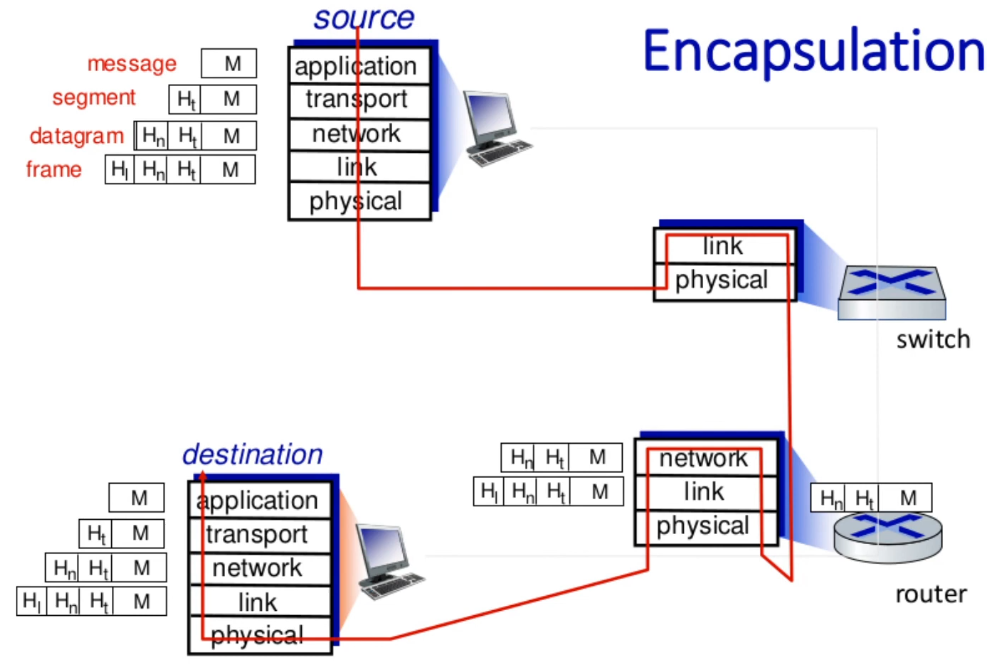
\includegraphics[width=0.4\textwidth]{img/cap-01/encapsulamento.png}
            \caption{Processo de encapsulamento nas camadas de protocolos.}
        \end{figure}
    
    \end{itemize}
